\begin{inhalt}
\renewcommand*\chapterpagestyle{scrheadings}

\section{Website}

Für das Bauen einer Website muss sich zuerst gefragt werden mit was man eigentlich eine Website baut. Dafür gibt es die verschiedene Möglichkeiten. In diesem Fall wurde NextJS genommen da es eines der meistgenutzten Frameworks \cite{SurveyStackOverflow} für JavaScript ist.

\vspace{1cm}

\textbf{Frontend}

Der Großteil des Frontends wird zunächst in Obsidian mithilfe des Excalidraw-Plugins entworfen, um zu veranschaulichen, wie eine Seite aussehen könnte.

\begin{figure}[!htb] 
\centering 
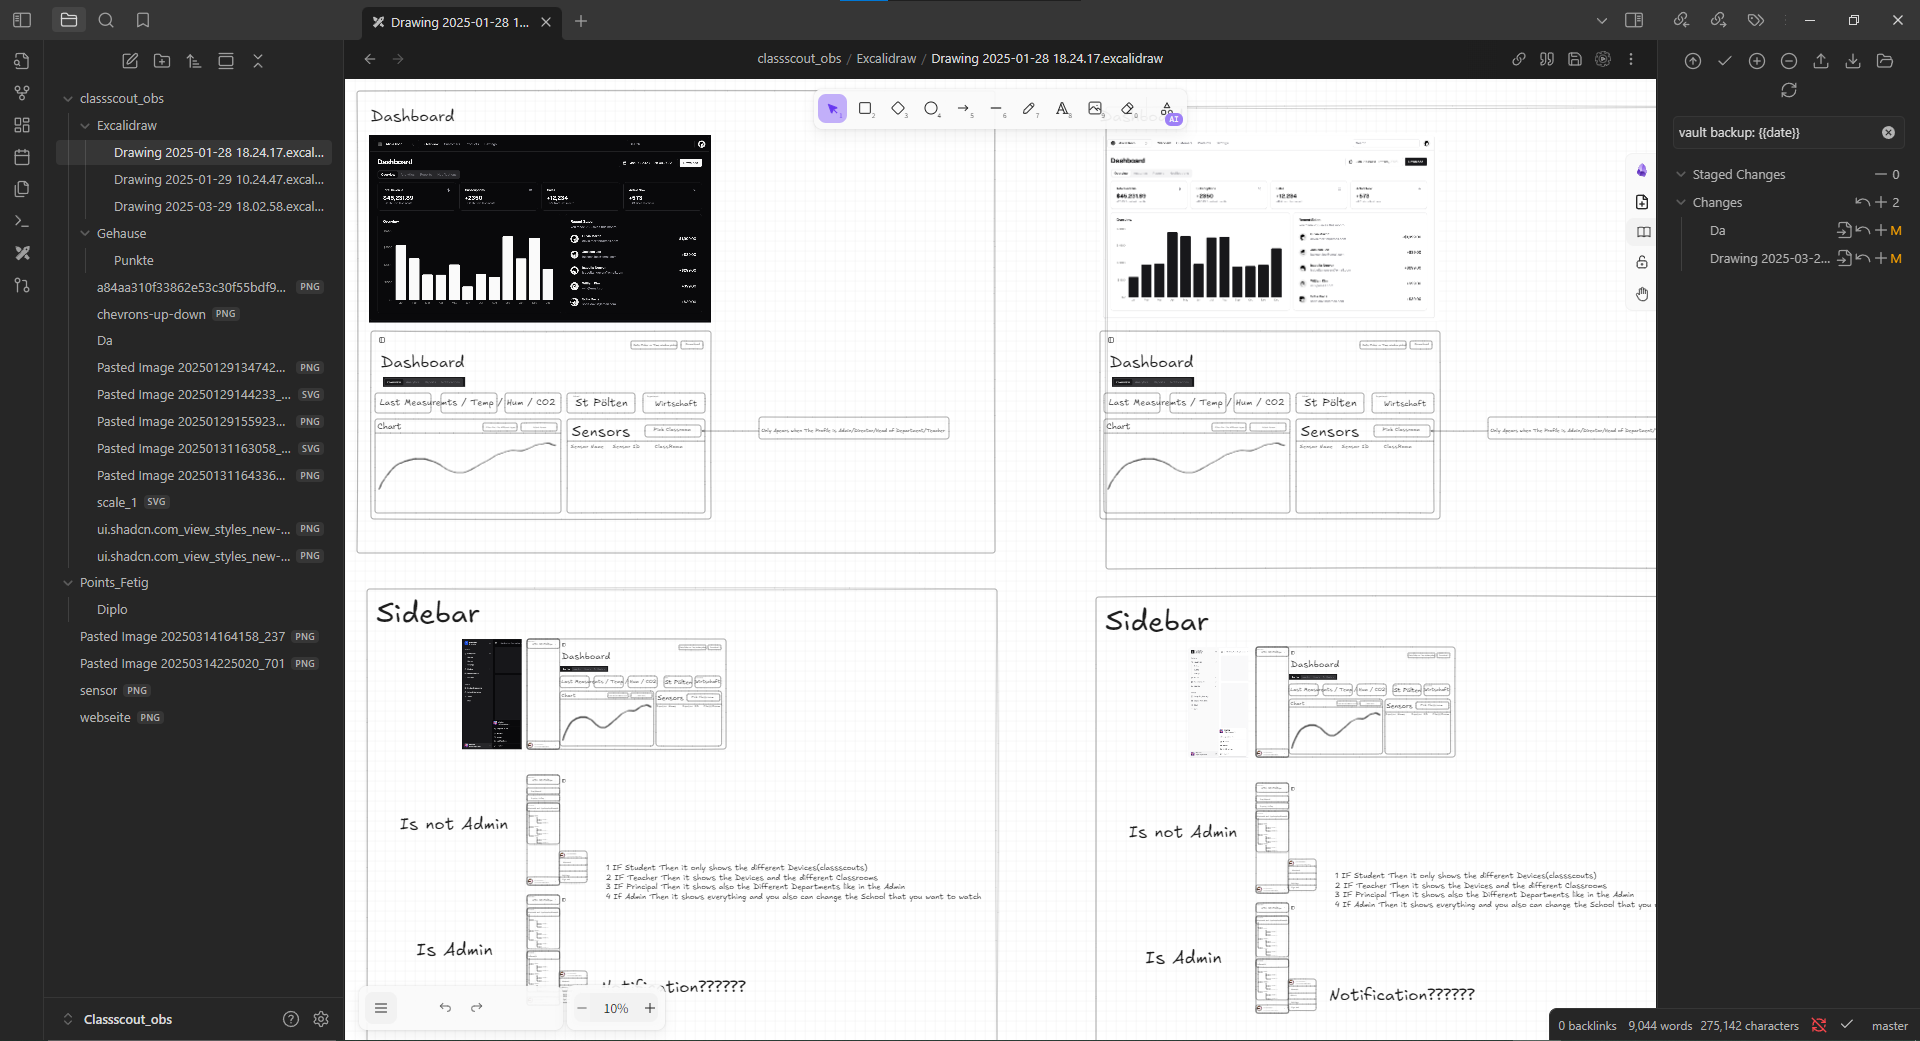
\includegraphics[width=1\textwidth]{files/Thomas/pics/Design-Grundlagen/image.png} 
\caption[Obsidan mit dem Excalidraw-Plugin geöffnet]{Obsidan mit dem Excalidraw-Plugin geöffnet} 
\label{fig:gehaeuse_internet_bild} 
\end{figure}

\newpage
\subsection{Dashboard}

Im Rahmen dieser Diplomarbeit wurde das Dashboard unter Berücksichtigung moderner Designansätze entwickelt. Es orientiert sich an dem Beispiel auf der Shadcn-Website \cite{ShadCNDashboard}, wobei die Gestaltung den spezifischen Anforderungen unseres Projekts angepasst wurde.

\begin{figure}[!htb] 
\centering 
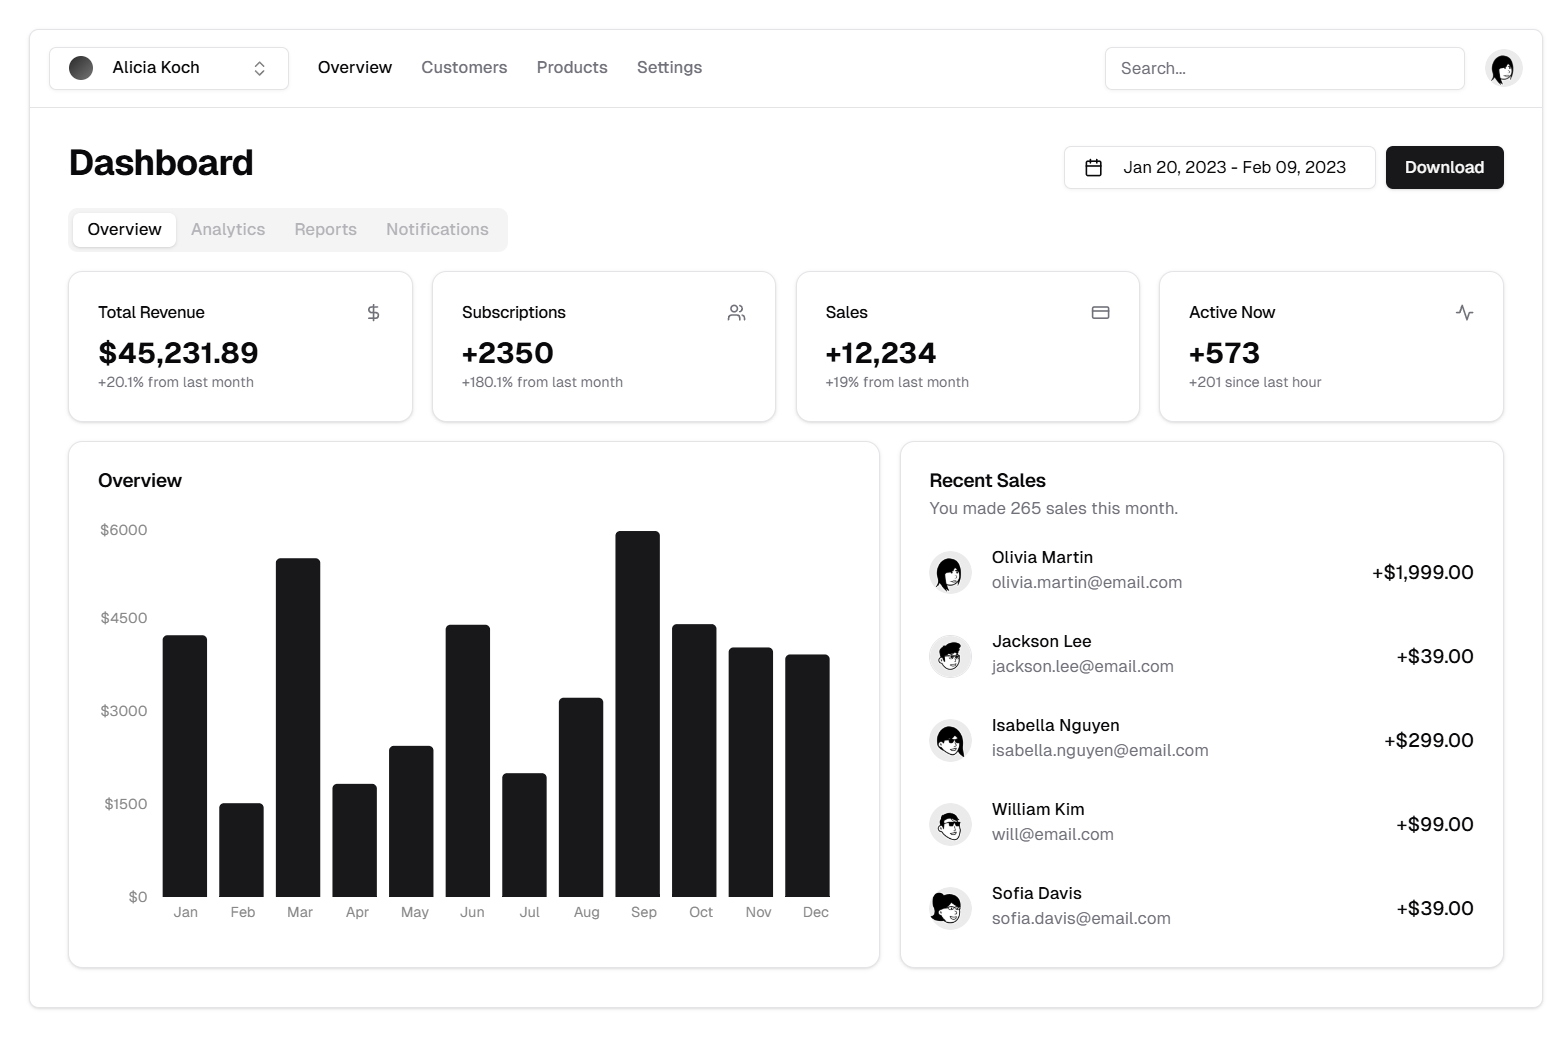
\includegraphics[width=0.85\textwidth]{files/Thomas/pics/Design-Grundlagen/Frontend/Dashboard/dashboard.png} 
\caption[Shadcn Beispiel Dashboard]{Shadcn Beispiel Dashboard} 
\label{fig:gehaeuse_internet_bild} 
\end{figure}

\vspace{-0.5cm}

\begin{figure}[!htb] 
\centering 
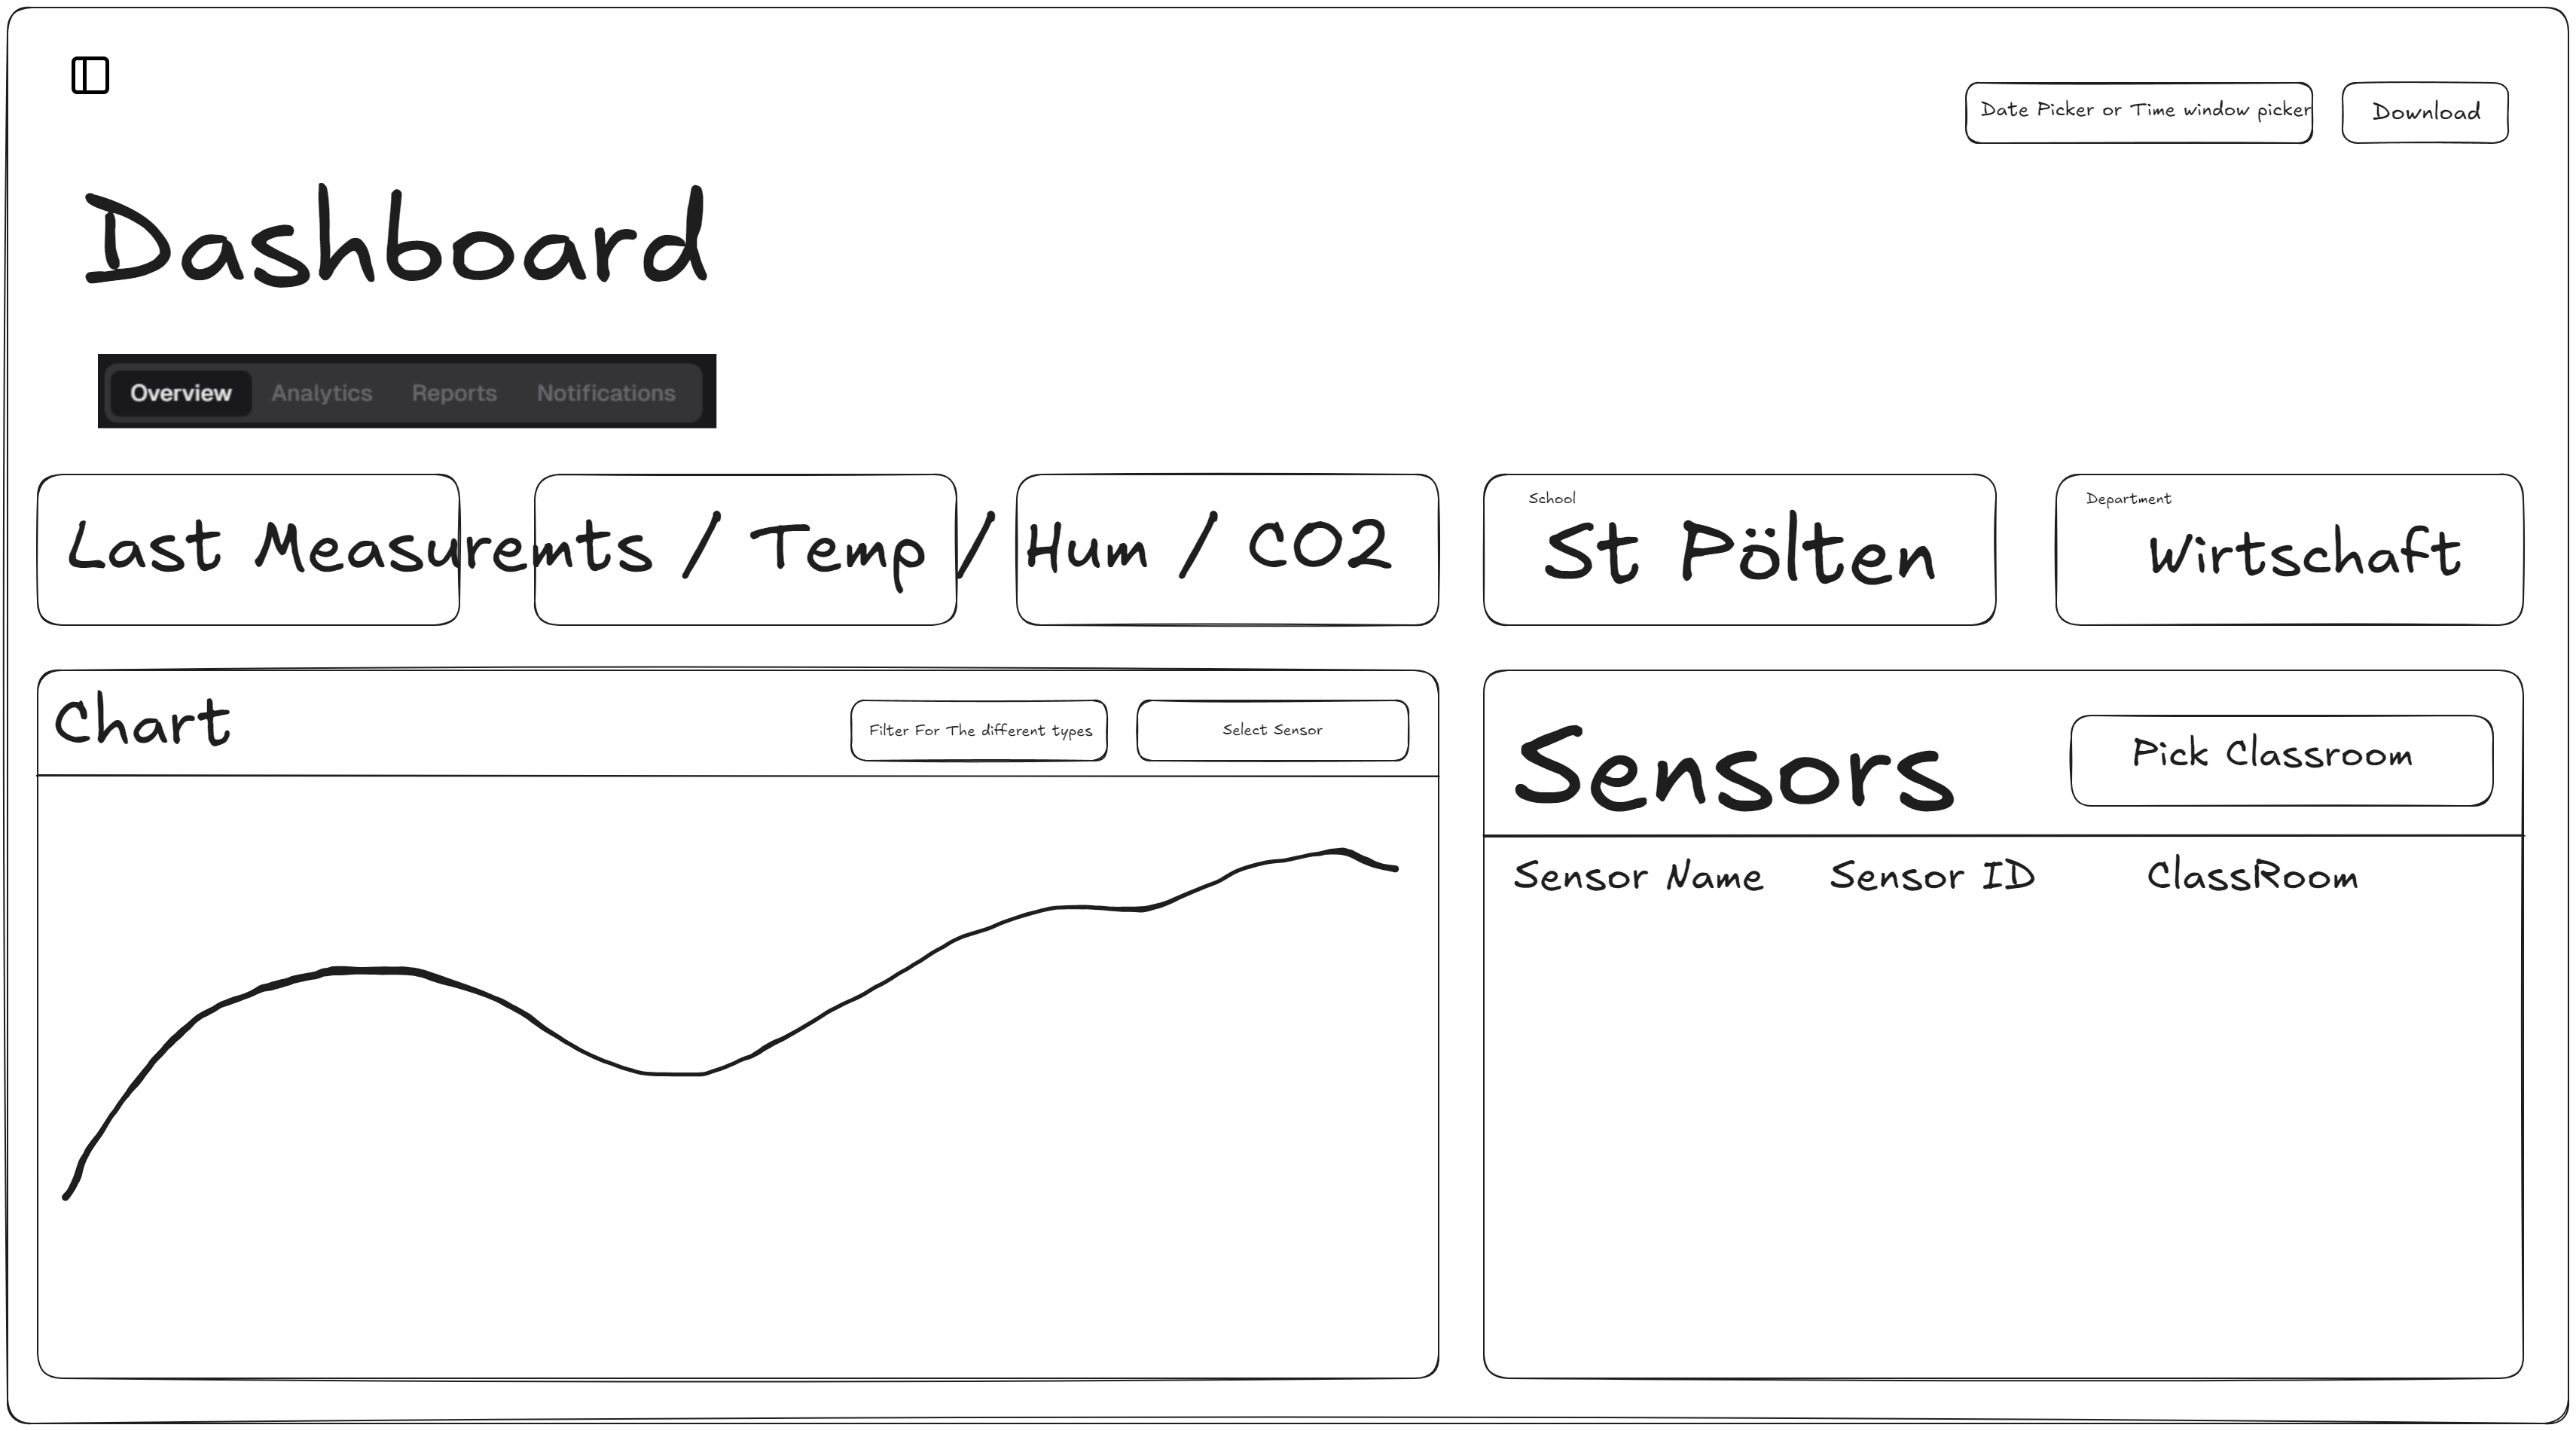
\includegraphics[width=0.85\textwidth]{files/Thomas/pics/Design-Grundlagen/Frontend/Dashboard/Dashboard-Draw.png} 
\caption[Umdesignte Dashboard]{Umdesignte Dashboard} 
\label{fig:gehaeuse_internet_bild} 
\end{figure}

\newpage

\subsection{Administrationsseiten}
\label{ref:Administrationsseiten}

Für die Entwicklung der Administrationsseiten wurde ein Konzept erarbeitet, das eine strukturierte und benutzerfreundliche Verwaltung der unterschiedlichen Datensätze ermöglicht. Auf der linken Seite wird eine Tabelle angezeigt, in der alle relevanten Einträge übersichtlich dargestellt werden. Auf der rechten Seite befindet sich eine Komponente zur Erstellung neuer Datensätze, welche die jeweiligen Tabellen ergänzt. Das System umfasst dabei separate Tabellen für Schulen, Abteilungen, Klassen, Sensoren und Benutzer, um eine differenzierte und effiziente Datenverwaltung zu gewährleisten. Zusätzlich erfolgt auf der Schul-Administrationsseite eine Visualisierung der Schulstandorte mittels einer Kartenansicht, um die räumliche Verteilung der Schulen anschaulich darzustellen.

\vspace{1cm}


\begin{figure}[!htb] 
\centering 
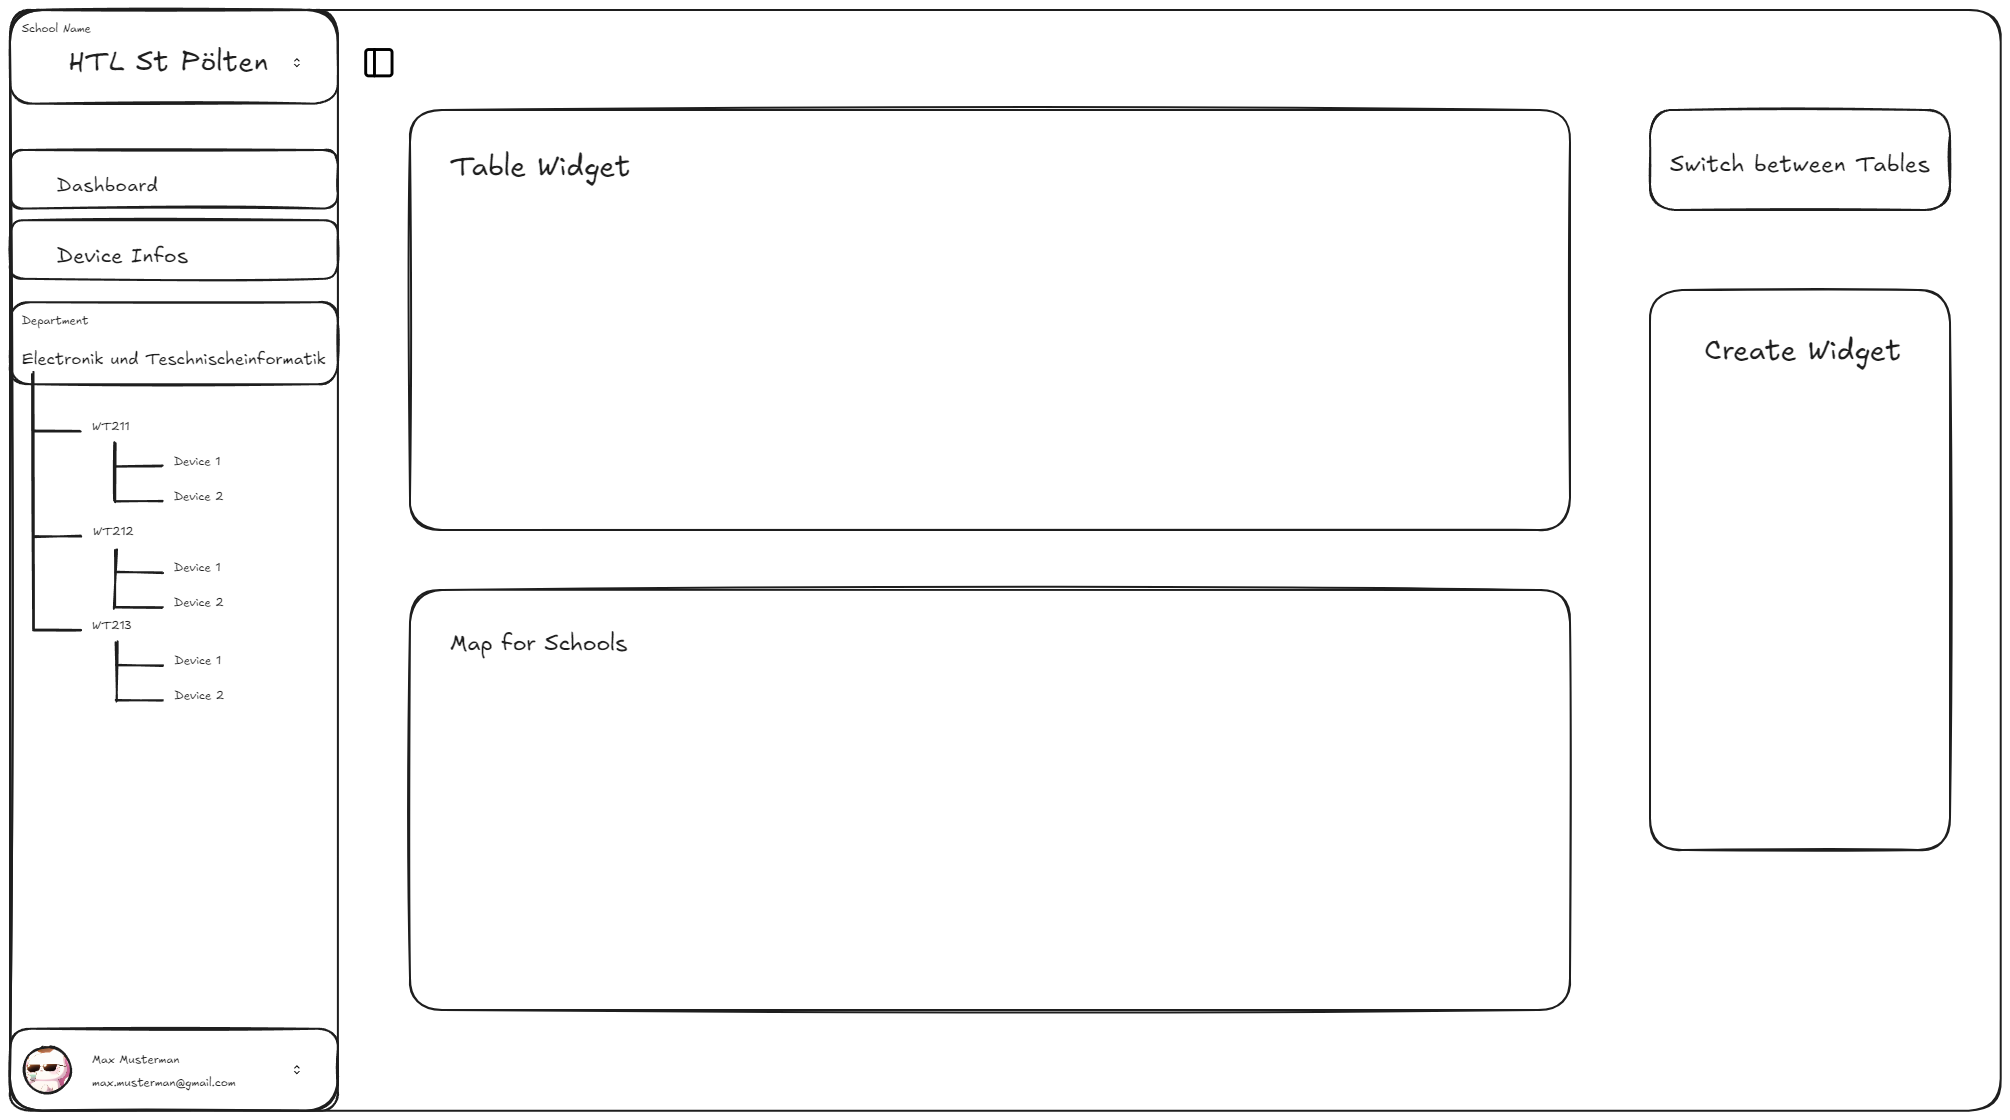
\includegraphics[width=1\textwidth]{files/Thomas/pics/Design-Grundlagen/Frontend/AdminSeite/AdminSeite-Draw.png} 
\caption[Beispiel einer Admin-Seite]{Beispiel einer Admin-Seite} 
\label{fig:gehaeuse_internet_bild} 
\end{figure}

\newpage

\subsection{Seitenleiste}

Die Seitenleiste \cite{ShadCNSidebar} wurde aufgrund ihrer optimalen Form ausgewählt, um den Benutzeraccount übersichtlich darzustellen. Zudem ermöglicht sie es Administratoren, den aktuell ausgewählten Schulstandort zu wechseln, wodurch eine bessere Übersicht über die laufenden Prozesse erzielt wird. Unterhalb dieses Bereichs werden sämtliche Abteilungen mitsamt den zugehörigen Klassen und Sensoren angezeigt. Die Sichtbarkeit einzelner Abteilungen richtet sich nach der jeweiligen Benutzerrolle: Während Administratoren sowie Schulleiter (Direktoren) alle Abteilungen mit den entsprechenden Klassen und Geräten einsehen können, erhalten Lehrkräfte ausschließlich Zugriff auf die Abteilung, in der sie tätig sind, und Schülerinnen sowie Schüler sehen lediglich ihre eigene Klasse.


%\begin{figure}[H]
%\centering
%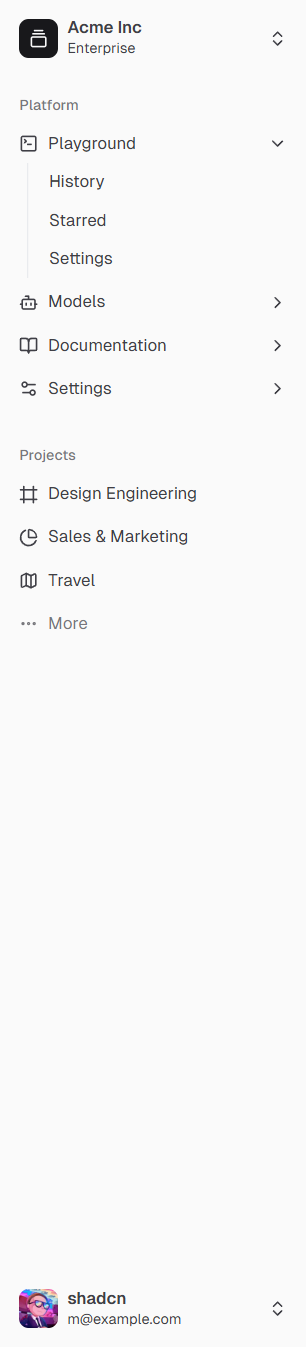
\includegraphics[width=0.3\textwidth]{files/Thomas/pics/Design-Grundlagen/Frontend/Sidebar/sidebar.png}
%\caption[Beispiel einer Admin-Tabelle}
%\label{fig:gehaeuse_internet_bild]{Beispiel einer Admin-Tabelle}
%\label{fig:gehaeuse_internet_bild}
%\end{figure}

\begin{figure}[!htb] 
\centering 
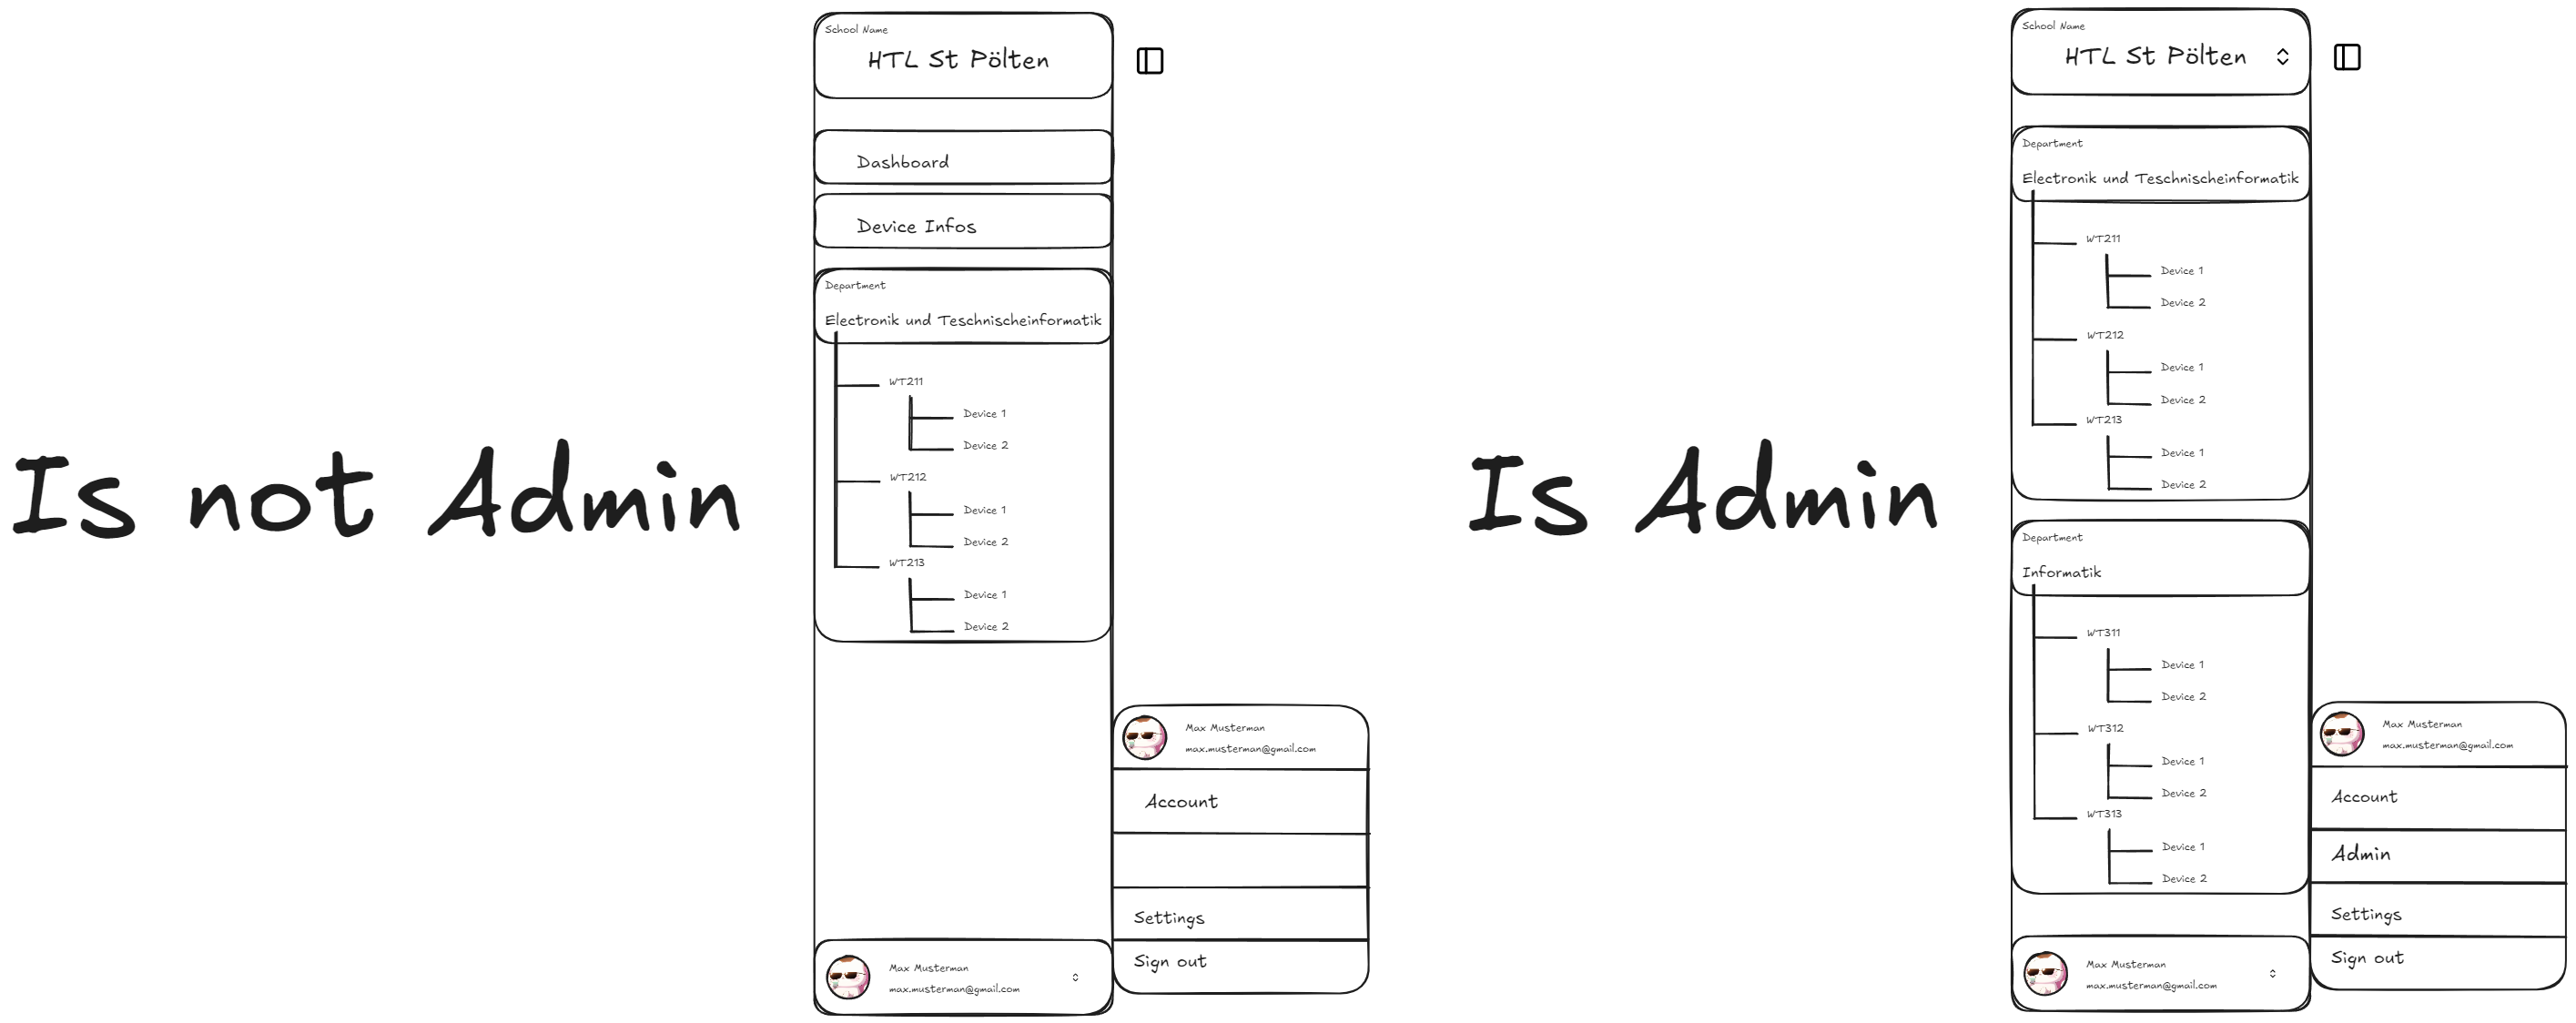
\includegraphics[width=0.75\textwidth]{files/Thomas/pics/Design-Grundlagen/Frontend/Sidebar/sidebar-adminvsnotadmin.png} 
\caption[Seitenleiste Design Vergleich]{Seitenleiste Design Vergleich} 
\label{fig:gehaeuse_internet_bild} 
\end{figure}


Wird ein Sensor ausgewählt, gelangt der Benutzer auf das zugehörige Dashboard, welches detaillierte Informationen zu dem jeweiligen Sensor, der Klasse oder der Abteilung bereitstellt. Im unteren Bereich der Seitenleiste befindet sich zudem das Profilbild, ergänzt durch den Benutzernamen und die E-Mail-Adresse. Beim Anklicken dieses Elements öffnet sich eine Auswahlliste mit weiteren Optionen. Diese umfasst zum einen die Möglichkeit, über eine dedizierte Account-Seite den Account zu verwalten – beispielsweise den Namen, das Profilbild und den Benutzernamen zu ändern – zum anderen den Zugriff auf die in Abschnitt \ref{ref:Administrationsseiten} erläuterten Administrationsseiten sowie eine Einstellungsseite. Auf dieser können unter anderem persönliche Schlüssel für das zugeordnete Gerät sowie weitere Funktionen eingesehen werden. Abschließend steht ein Logout-Button zur Verfügung, der den Benutzer aus dem System abmeldet und zur Login-Seite zurückführt.

\begin{figure}[!htb] 
\centering 
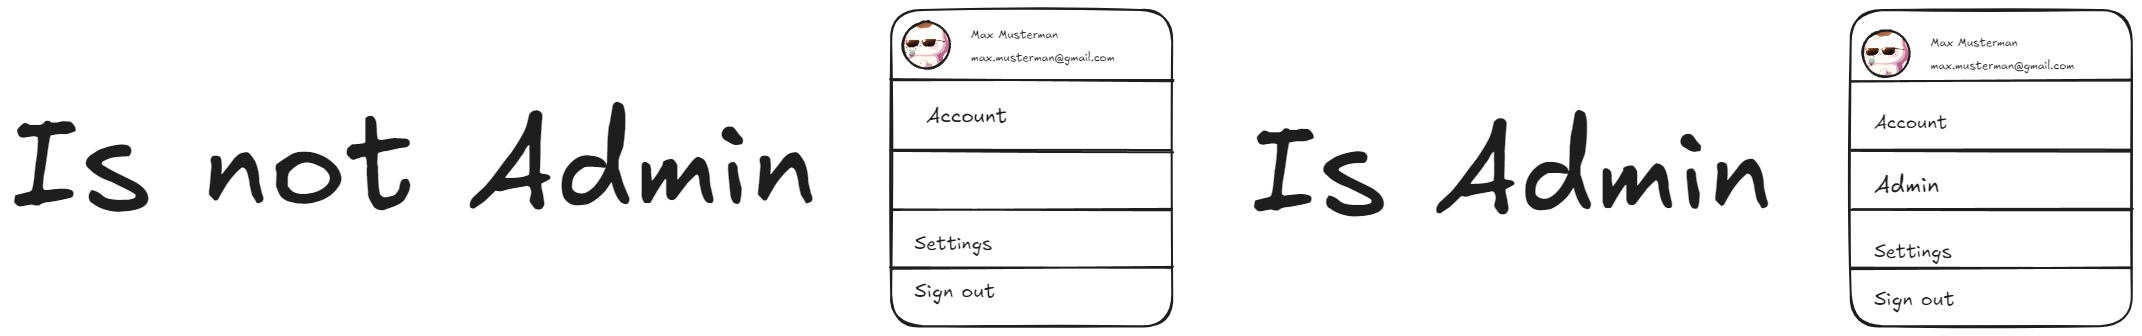
\includegraphics[width=0.7\textwidth]{files/Thomas/pics/Design-Grundlagen/Frontend/Sidebar/sidebar-nav-user-adminvsnotadmin.png} 
\caption[Benutzer Navigations Vergleich]{Benutzer Navigations Vergleich} 
\label{fig:gehaeuse_internet_bild} 
\end{figure}

\newpage

































\subsection{Backend} \label{sec:Backend-Design}
\label{ref:backend_design}

Im Folgenden wird das Design des Backends erläutert. Das System ist in der Lage, verschiedene Messwerte zu verarbeiten, darunter CO\textsubscript{2}-Konzentrationen, Feuchtigkeitswerte, Temperaturwerte, Gaswiderstandswerte sowie einen Zeitstempel. Diese Daten werden im JSON-Format vom Backend empfangen. Zur Sicherstellung einer einheitlichen Datenstruktur wurde das folgende JSON-Schema definiert:

\begin{lstlisting}[style=myjson]
{
    "measured_at": "2024-10-23T12:29:02.379+00:00",
    "co2": 6,
    "hum": 7,
    "temp": 8,
    "gasres": 9
}
\end{lstlisting}

\vspace{3cm}

Zur eindeutigen Identifizierung der einzelnen Sensoren wird beim Anlegen eines Sensors auf der Administrationsseite stets eine Sensor-ID generiert. Diese dient als einzigartiger Identifikator, der es ermöglicht, die Messdaten den entsprechenden Sensoren zuzuordnen. Dementsprechend wird die Sensor-ID in den JSON-Daten mitübertragen:

\begin{lstlisting}[style=myjson]
{
    "token": "d192f90b-a5b8-4767-b5af-59ec40fe03c2",
    "measured_at": "2024-10-23T12:29:02.379+00:00",
    "co2": 6,
    "hum": 7,
    "temp": 8,
    "gasres": 9
}
\end{lstlisting}

\newpage

Ein Problem tritt auf, wenn mehrere Messdaten gleichzeitig versendet werden sollen, da mehr Messpunkte erfasst werden, als in einer einzelnen Übertragung enthalten sein können. Zur Lösung dieses Problems wurde ein erweitertes JSON-Format entwickelt, das die Übermittlung mehrerer Messdatensätze in einer einzigen Nachricht ermöglicht:

\begin{lstlisting}[style=myjson]
{
    "token": "d192f90b-a5b8-4767-b5af-59ec40fe03c2",
    "data": [
        {
            "measured_at": "2024-10-23T12:28:02.379+00:00",
            "co2": 3,
            "hum": 4,
            "temp": 5,
            "gasres": 6
        },
        {
            "measured_at": "2024-10-23T12:29:02.379+00:00",
            "co2": 6,
            "hum": 7,
            "temp": 8,
            "gasres": 9
        },
        {
            "measured_at": "2024-10-23T12:30:02.379+00:00",
            "co2": 9,
            "hum": 10,
            "temp": 11,
            "gasres": 12
        }
    ]
}
\end{lstlisting}

Mit diesem erweiterten Datenformat ist das Backend in der Lage, die empfangenen Messdaten effizient in der Datenbank zu speichern.

\newpage


\section{Datenbank}

\label{ref:profile-table-design}
Bei der Planung der Datenbankstruktur wurde zunächst festgestellt, dass Supabase zwar über die integrierte Authentifizierungstabelle theoretisch benutzerspezifische Daten abspeichern könnte, dies jedoch nicht vorgesehen ist. Aus diesem Grund wurde entschieden, eine eigene Tabelle für Benutzer anzulegen.

\begin{figure}[!htb]
  \centering
  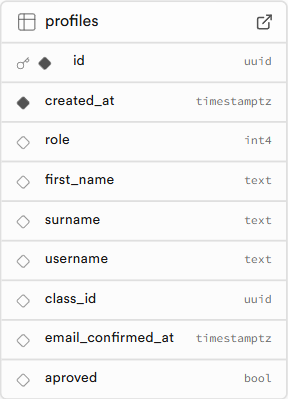
\includegraphics[scale=0.5]{files/Thomas/pics/Datenbank_Design/profiles.png}
  \caption[Benutzertabelle der Datenbank]{Tabelle zur Speicherung der Benutzerdaten}
  \label{fig:profiles_tabelle}
\end{figure}

Im nächsten Schritt musste eine sinnvolle Struktur für die Verwaltung der Sensoren entworfen werden. Da das System nicht ausschließlich für die HTL St. Pölten vorgesehen ist, sondern auch von anderen Bildungseinrichtungen genutzt werden könnte, wurde die Datenbank entsprechend erweitert. Es wurde eine Tabelle \textit{Schools} erstellt, um mehrere Schulen abbilden zu können.

\begin{figure}[!htb]
  \centering
  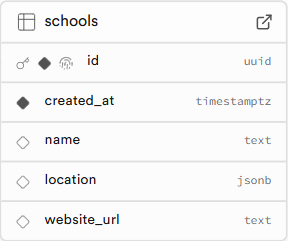
\includegraphics[scale=0.5]{files/Thomas/pics/Datenbank_Design/school.png}
  \caption[Schultabelle der Datenbank]{Schultabelle}
  \label{fig:schools_tabelle}
\end{figure}

\newpage

Da eine Schule in verschiedene Abteilungen untergliedert ist, wurden zusätzlich die Tabellen \textit{Departments} (Abteilungen) sowie \textit{Classes} (Klassen) angelegt. Diese Struktur ermöglicht eine klare Zuordnung und Verwaltung der Sensoren auf Klassen- bzw. Abteilungsebene innerhalb der jeweiligen Schule.

\begin{figure}[!htb]
  \centering
  \begin{subfigure}[b]{0.45\textwidth}
    \centering
    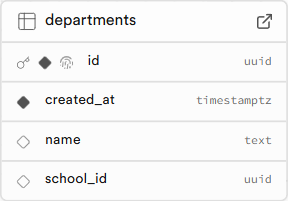
\includegraphics[scale=0.45]{files/Thomas/pics/Datenbank_Design/departments.png}
    \caption[Tabelle Departments]{Abteilungenstabelle}
    \label{fig:departments_tabelle}
  \end{subfigure}
  \hfill
  \begin{subfigure}[b]{0.45\textwidth}
    \centering
    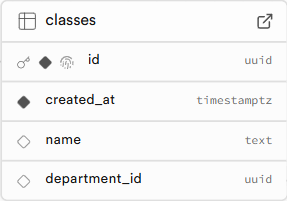
\includegraphics[scale=0.45]{files/Thomas/pics/Datenbank_Design/classes.png}
    \caption[Tabelle Classes]{Klassentabelle}
    \label{fig:classes_tabelle}
  \end{subfigure}
  \caption[Abteilungs- und Klassentabellen]{Datenbankstruktur von Klassen und Abteilungen}
  \label{fig:departments_classes}
\end{figure}

Für die eigentlichen Sensordaten wurden zwei weitere Tabellen erstellt: \textit{Sensors} und \textit{Sensor\_Readings}. Die Trennung dieser Informationen ist notwendig, da bei einer Speicherung der Messwerte direkt in der \textit{Sensors}-Tabelle lediglich die aktuellen Werte abrufbar wären. Da jedoch geplant ist, die historischen Messwerte in Form von Zeitdiagrammen darzustellen, müssen diese dauerhaft gespeichert werden. Aus diesem Grund enthält die Tabelle \textit{Sensor\_Readings} zeitlich zuordenbare Einzelmessungen, welche sich eindeutig einem Sensor zuordnen lassen.

\begin{figure}[!htb]
  \centering
  \begin{subfigure}[b]{0.45\textwidth}
    \centering
    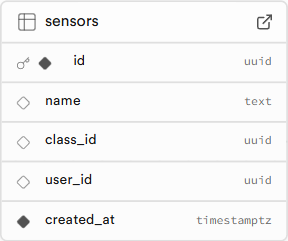
\includegraphics[scale=0.45]{files/Thomas/pics/Datenbank_Design/sensors.png}
    \caption[Tabelle Sensors]{Sensorentabelle}
    \label{fig:sensors_tabelle}
  \end{subfigure}
  \hfill
  \begin{subfigure}[b]{0.45\textwidth}
    \centering
    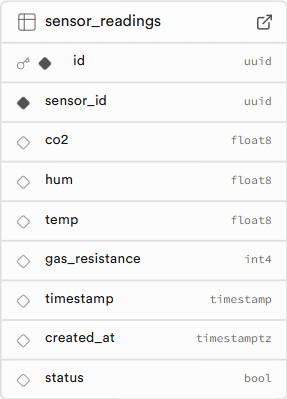
\includegraphics[scale=0.45]{files/Thomas/pics/Datenbank_Design/sensor_readings.png}
    \caption[Tabelle Sensor Readings]{Messwerttabelle}
    \label{fig:sensor_readings_tabelle}
  \end{subfigure}
  \caption[Sensor- und Messwerttabellen]{Datenbankstruktur von Sensoren und Messwerten}
  \label{fig:sensors_sensor_readings}
\end{figure}

\newpage

\begin{sidewaysfigure}[!htb]
  \centering
  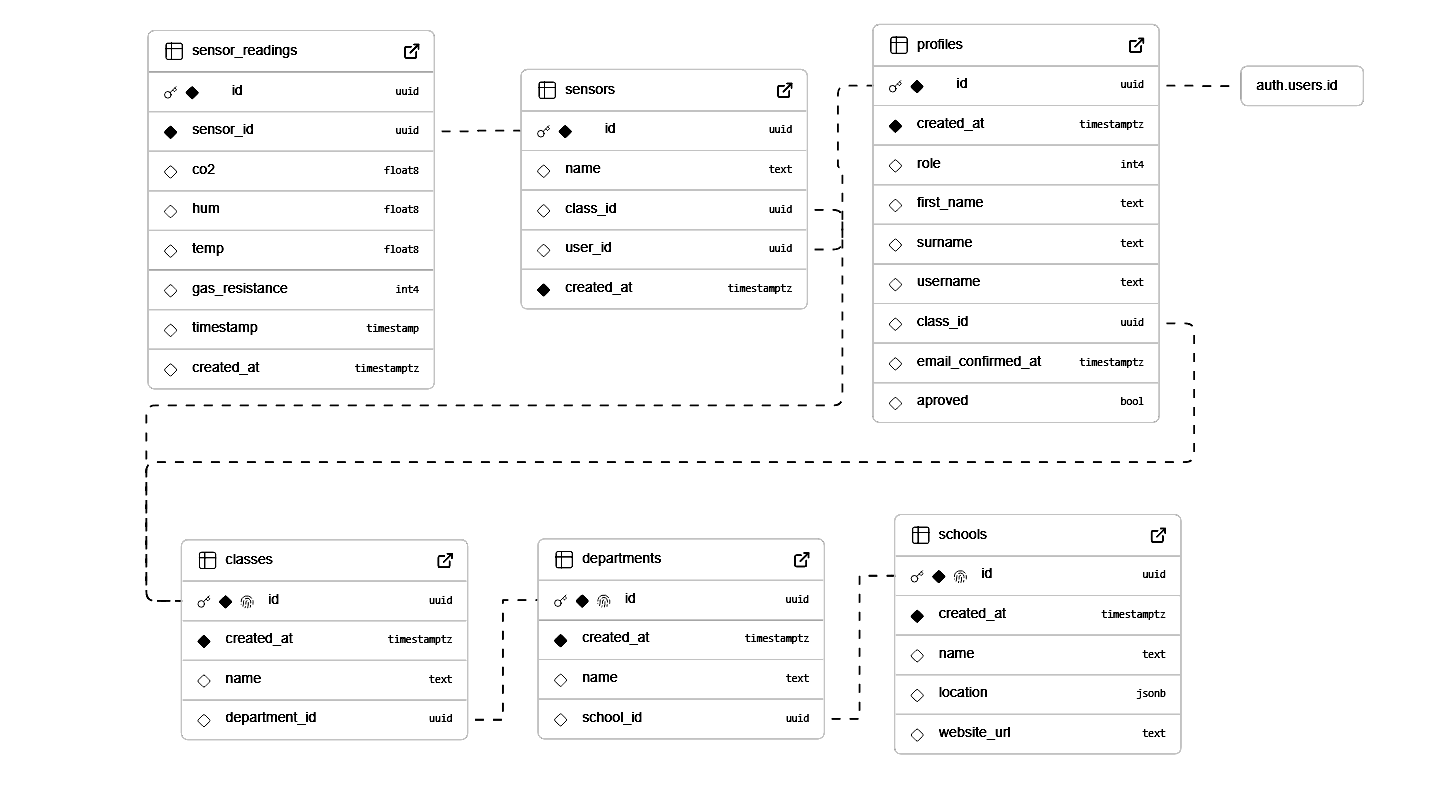
\includegraphics[scale=0.45]{files/Thomas/pics/output.png}
  \caption[Gesamtübersicht der Datenbankstruktur]{Gesamtdiagramm der Datenbankstruktur mit allen relevanten Tabellen und Verknüpfungen.}
  \label{fig:db_gesamt}
\end{sidewaysfigure}

\clearpage
\newpage

\section{Gehäuse}

Zunächst wurde eine umfassende Recherche im Internet durchgeführt, um bestehende Designvarianten zu identifizieren. Dabei wurde ein Design entdeckt, das den Anforderungen entsprach \cite{TemuGehaeuseURL}(\ref{fig:gehaeuse_internet_bild}).

\vspace{0.15cm}

Um eine praktikable Lösung zu entwickeln, wurde ein alternativer Ansatz verfolgt: Es sollte ein Gehäuse konzipiert werden, das sich leicht auseinandernehmen lässt. Ergänzende Recherchen auf YouTube \cite{GehaeuseYoutubeClipsURL} ergaben, dass der Einsatz von Klammern als Verbindungselemente eine Möglichkeit darstellt, das Gehäuse sicher zusammenzuhalten und gleichzeitig eine einfache Demontage zu gewährleisten.

\vspace{0.15cm}

Diese Methode bietet den Vorteil, dass das Gehäuse nicht nur robust zusammengebaut ist, sondern auch bei Bedarf zügig geöffnet werden kann, um Wartungsarbeiten durchzuführen oder interne Komponenten auszutauschen.

\begin{figure}[!htb]
\centering
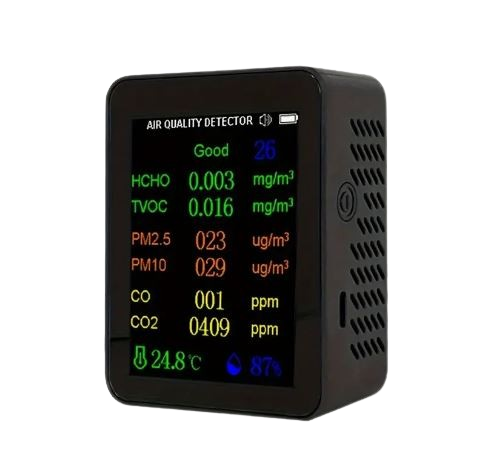
\includegraphics[width=0.75\textwidth]{files/Thomas/pics/new/Temu-removebg-preview.png}
\caption[Gehäuse mit optimiertem Airflow, aus der Internetrecherche \cite{TemuGehaeuse}]{Gehäuse mit optimiertem Airflow, aus der Internetrecherche \cite{TemuGehaeuse}}
\label{fig:gehaeuse_internet_bild}
\end{figure}



\end{inhalt}